\documentclass{beamer}

\usepackage[utf8]{inputenc}
\usepackage{default}
\usepackage{graphicx}


\title{OL3-Cesium: 3D for OpenLayers}
\author{Guillaume Beraudo}
\institute{Opensource Engineer\\Camptocamp, Switzerland}
\date{FOSDEM 2016, January 31\textsuperscript{st}}
\subject{OL3-Cesium FOSDEM 2016 talk}

\hypersetup{colorlinks,urlcolor=blue}
\setbeamertemplate{footline}[text line]{%
  \parbox{\linewidth}{\vspace*{-8pt}OL3-Cesium\hfill\insertshortauthor, FOSDEM 2016}}
\setbeamertemplate{navigation symbols}{}

\begin{document}

  \begin{frame}
    \titlepage
  \end{frame}

  \begin{frame}
       \frametitle{Goal}
    \begin{center}
        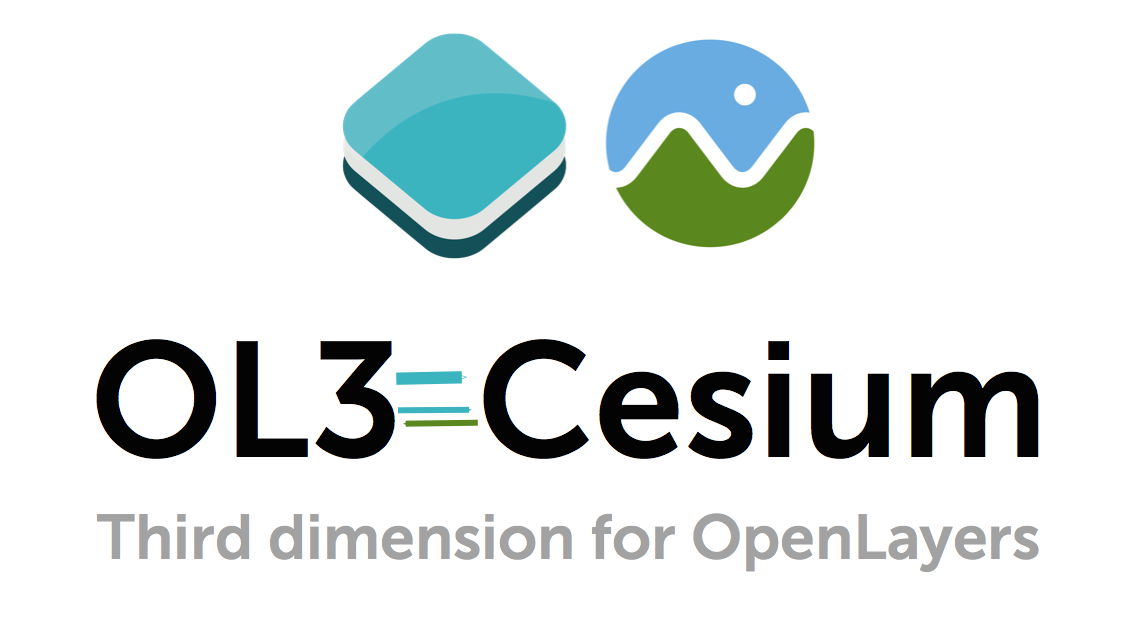
\includegraphics[width=.3\linewidth]{./ol3-cesium-wide_arrows.png}
        % ol3-cesium-wide_arrows.png: 1146x638 pixel, 72dpi, 40.43x22.51 cm, bb=0 0 1146 638
    \end{center}

      JS library to synchronize an OL3 map and a Cesium 3D globe
  \end{frame}


  \begin{frame}
    \frametitle{OL3 - 2D map, pixel perfect, Swiss projection}
		\begin{center}
		  \includegraphics[width=1.0 \linewidth]{./vtt_2d.png}
		    % vtt_2d.png: 0x0 pixel, 300dpi, 0.00x0.00 cm, bb=
		\end{center}
  \end{frame}

  \begin{frame}
    \frametitle{Cesium - 3D globe, WEBGL, latlong}
		\begin{center}
		  \includegraphics[width=1.0 \linewidth]{./vtt_3d2.png}
		    % vtt_3d2.png: 0x0 pixel, 300dpi, 0.00x0.00 cm, bb=
		\end{center}
    \href{https://map.schweizmobil.ch/?cesium&trackId=2149217}{Schweizmobil 3D}
  \end{frame}



  \begin{frame}
    \frametitle{Getting started}

    \begin{itemize}
      \item
        \small{\texttt{ol3d = new olcs.OLCesium(\{map: map\})}}
        \small{\texttt{ol3d.setEnabled(true)}}
        \pause
      \begin{itemize}
        \item A Cesium globe is created
          \pause
        \item Existing layers and view are synchronized
         \pause
        \item Some listeners are registered
          \pause
      \end{itemize}
      \item Demo
    \end{itemize}
  \end{frame}


  \begin{frame}
    \frametitle{Manipulate OL3, get the work done}
    \begin{itemize}
      \item Adding a new layer: \small{\texttt{myOl3Map.addLayer(...)}}
        \pause
      \item Adding a feature: \small{\texttt{myOl3Source.addFeature(...)}}
        \pause
      \item Removing a feature: \small{\texttt{myOl3Source.RemoveFeature(...)}}
        \pause
      \item Changing a feature style: \small{\texttt{myOl3Feature.setStyle(...)}}
    \end{itemize}
  \end{frame}


  \begin{frame}
    \frametitle{Keep in mind}
    \begin{itemize}
      \item Reprojection (mind rasters!, olcs.AbstractSynchronizer)
        \pause
      \item Features in 3D (mind polylines! clampToGround)
        \pause
      \item Clustering (\href{https://github.com/gberaudo/ol3-cluster-tool}{ol3-cluster-tool}, GPU decimation)
        \pause
      \item Fog (30\% bandwidth saving + less latency)
        \pause
      \item Eager/lazy loading (pay when you use)
        \pause
      \item Pausing renderloop (don't drain battery! CPU: 100\% $\rightarrow$ 5\%)
    \end{itemize}
  \end{frame}



  \begin{frame}
    \frametitle{Future}
    \vspace{-20pt}\begin{center}
      \includegraphics[width=0.9\linewidth]{./github2.png}
    \end{center}
    \begin{itemize}
      \item Keep up with Ol3 and Cesium pace
        \pause
      \item Client side reprojection?
        \pause
      \item Have ideas? Want to participate?
        \pause
      \item Thanks, questions?
    \end{itemize}
  \end{frame}

\end{document}
